% !TEX program = xelatex
\documentclass[UTF8,a4paper,10pt,fontset=windows]{ctexart}

\usepackage[a4paper,top=1.75cm,bottom=1.8cm,left=1.65cm,right=1.65cm,headheight=14pt]{geometry}
\usepackage{amsmath,amssymb,bm}
\usepackage{graphicx}
\usepackage{booktabs,array}
\usepackage{caption}
\usepackage{xcolor}
\usepackage{enumitem}
\usepackage{fancyhdr}
\usepackage{microtype}
\usepackage{hyperref}

\definecolor{AcademicBlue}{HTML}{245A7A}
\definecolor{TextGray}{HTML}{4A5560}
\hypersetup{hidelinks,pdftitle={让CLIP理解异常：AA-CLIP的零样本异常检测方法},pdfauthor={Rpc}}
\graphicspath{{assets/paper-figures/}}
\setlength{\columnsep}{0.72cm}
\setlength{\emergencystretch}{1.5em}
\setlength{\parindent}{2em}
\setlength{\parskip}{0pt}
\linespread{1.08}
\setlist{nosep,leftmargin=1.6em}
\captionsetup{font=small,labelfont=bf,labelsep=quad}
\ctexset{
  section={format=\large\bfseries\color{AcademicBlue},beforeskip=0.8em,afterskip=0.35em},
  subsection={format=\normalsize\bfseries,beforeskip=0.55em,afterskip=0.25em}
}

\pagestyle{fancy}
\fancyhf{}
\fancyhead[L]{\small\color{TextGray}AA-CLIP 论文转述}
\fancyhead[R]{\small\color{TextGray}Rpc}
\fancyfoot[C]{\small\thepage}
\renewcommand{\headrulewidth}{0.35pt}

\newcommand{\TN}{T_{N}}
\newcommand{\TA}{T_{A}}
\newcommand{\loss}{\mathcal{L}}

\begin{document}

\twocolumn[
\begin{@twocolumnfalse}
  \begin{center}
    {\LARGE\bfseries 让 CLIP 理解“异常”：AA-CLIP 的零样本异常检测方法\par}
    \vspace{0.35em}
    {\large\bfseries Teaching CLIP What ``Abnormal'' Means: A Review of AA-CLIP\par}
    \vspace{0.7em}
    {\normalsize Rpc\par}
    {\small 论文阅读与转述作业，2026 年 8 月 11 日\par}
  \end{center}

  \begin{abstract}
  零样本异常检测要求模型将从源类别获得的知识迁移到训练阶段未见的产品或医学影像类别。CLIP 具有较强的跨类别泛化能力，但其通用图文预训练并未建立稳定的“正常--异常”判别方向。本文转述 Ma 等人提出的 Anomaly-Aware CLIP（AA-CLIP）：该方法先在文本空间中解耦正常与异常语义，再利用所得文本锚点约束多尺度图像块特征。原始 CLIP 参数始终冻结，仅训练浅层残差适配器和投影层。跨 11 个工业与医学数据集的实验表明，AA-CLIP 在有限训练样本下仍能获得较强的图像级检测与像素级定位性能。本文进一步讨论其贡献边界：论文中的“零样本”指向未见目标类别迁移，并不等同于无需源域标注或完全无训练的异常检测。
  \end{abstract}
  \noindent\textbf{关键词：}零样本异常检测；CLIP；残差适配器；视觉语言模型；异常定位
  \vspace{0.9em}
\end{@twocolumnfalse}
]

\section{引言}

异常检测需要识别偏离正常分布的图像，并在分割任务中定位具体异常区域。传统方法通常依赖特定类别的训练数据；当缺陷或病灶稀少、形态多变时，为每个新类别重新建模的成本较高。CLIP 通过大规模图文对比学习建立共享特征空间，因而能够利用“正常物体”和“损坏物体”等文本提示执行零样本判断\cite{radford2021}。

然而，通用语义能力不等于异常判别能力。原始 CLIP 中，同一类别的正常与异常提示往往具有较高余弦相似度，明显缺陷的图像也可能更接近正常描述。Ma 等人将这一现象称为\textit{异常无感知}（anomaly unawareness）\cite{ma2025}。因此，问题并非只需寻找更复杂的提示词，而是要让共享空间真正包含“是否异常”的判别方向，同时避免破坏 CLIP 已有的类别知识。

\section{AA-CLIP 方法}

\subsection{受控残差适配}

AA-CLIP 冻结 CLIP 主干，在文本与视觉编码器的前若干 Transformer 层后插入轻量残差适配器。第 $i$ 层特征 $x^i$ 首先经过线性变换、激活和归一化，再与原特征加权融合：
\begin{align}
x_{\mathrm{res}}^i &= \operatorname{Norm}\!\left(\operatorname{Act}(W^i x^i)\right), \\
x_{\mathrm{enh}}^i &= \lambda x_{\mathrm{res}}^i+(1-\lambda)x^i .
\end{align}
论文设置 $\lambda=0.1$，使原始表征占据主导，只注入少量异常检测知识。与直接微调整个编码器相比，该结构更有利于保留跨类别泛化能力。

\subsection{阶段一：解耦文本锚点}

第一阶段冻结视觉编码器，只训练文本侧浅层适配器和最终投影层。正常提示与异常提示分别被编码并求平均，得到文本锚点 $\TN$ 与 $\TA$。二者通过图像级二分类损失和像素级 Dice、Focal 损失与训练图像对齐：
\begin{equation}
\loss_{\mathrm{align}}
=\loss_{\mathrm{cls}}+\loss_{\mathrm{seg}}.
\end{equation}
为减少正常与异常语义的相关性，作者加入解耦损失
\begin{equation}
\loss_{\mathrm{dis}}=\left|\langle \TN,\TA\rangle\right|^2,
\end{equation}
最终目标为 $\loss_{\mathrm{total}}=\loss_{\mathrm{align}}+\gamma\loss_{\mathrm{dis}}$。该过程将“正常--异常”差异显式写入文本编码器，而非继续依赖原始 CLIP 中较模糊的提示嵌入。

\subsection{阶段二：对齐图像块特征}

第二阶段固定已经适配好的文本编码器，在视觉编码器浅层训练残差适配器。模型从第 6、12、18、24 层提取不同粒度的图像块特征 $F^i$，经投影后求和：
\begin{equation}
V_{\mathrm{patch}}=\sum_{i=1}^{4}\operatorname{Proj}_{i}(F^i).
\end{equation}
$V_{\mathrm{patch}}$ 与 $[\TN,\TA]$ 的余弦相似度形成像素级预测图；全局图像特征则用于图像级二分类。由于视觉侧追随的是第一阶段已经分离的语义锚点，定位获得了更明确的监督方向。

\begin{figure*}[t]
  \centering
  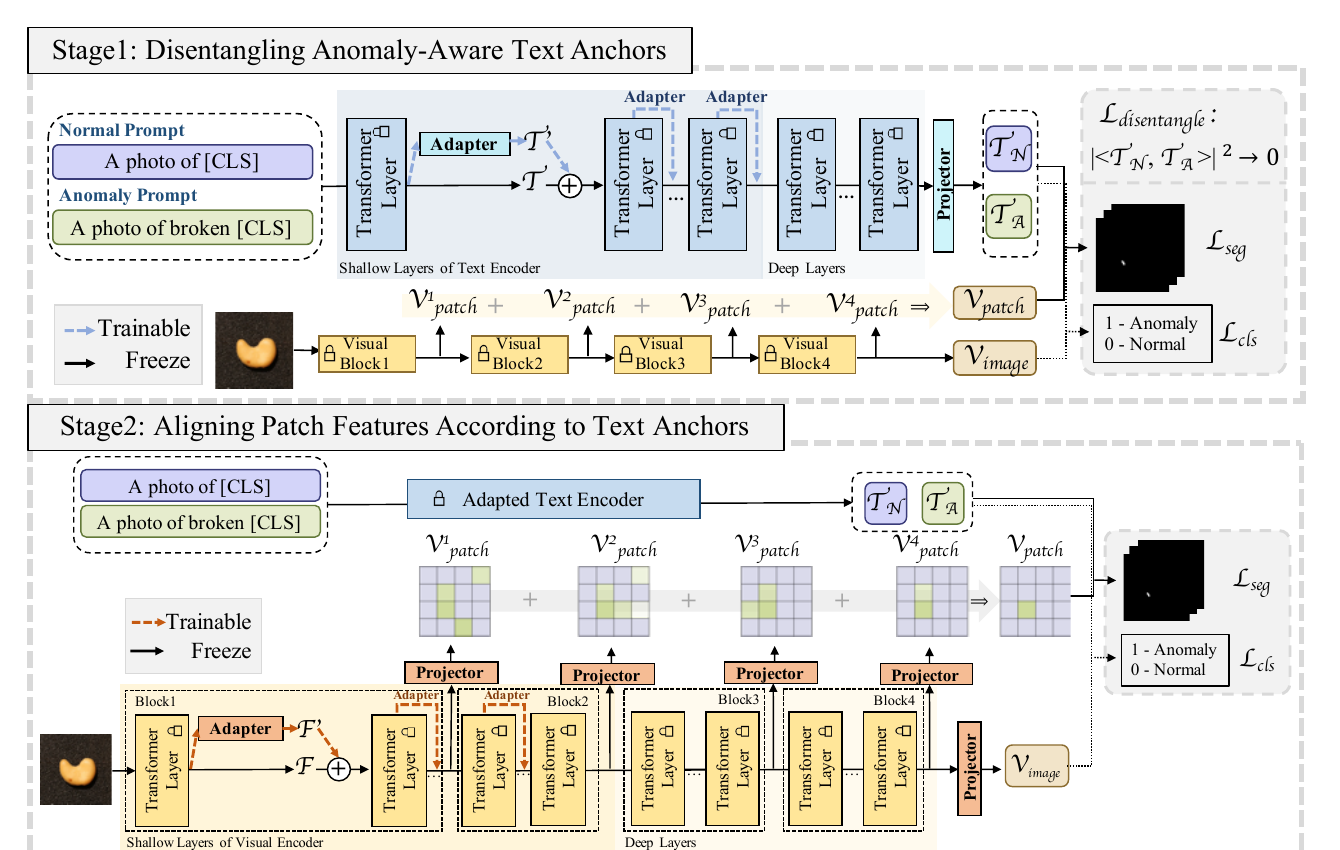
\includegraphics[width=0.91\textwidth]{fig4_pipeline.png}
  \caption{AA-CLIP 两阶段训练流程。阶段一适配文本空间并构建正常/异常锚点；阶段二固定文本锚点并对齐多尺度图像块特征。图片裁剪自原论文 Fig.~4，遵循 CC BY 4.0。}
  \label{fig:pipeline}
\end{figure*}

\section{实验与结果}

\subsection{实验设置}

作者在 MVTec AD、VisA、BTAD、MPDD 四个工业数据集，以及脑部 MRI、肝脏 CT、视网膜 OCT 和四个结肠息肉数据集上评估模型。训练数据规模包括每类 2、16、64 个样本和完整数据；测试类别与训练类别不同。骨干为 OpenCLIP ViT-L/14，输入分辨率为 $518\times518$。评价指标为图像级和像素级 AUROC。

需要强调的是，2-shot 设置仍包含正常与异常样本，训练阶段也使用图像级标签和像素掩膜。因此，此处的零样本描述的是\textit{目标类别未见}，而不是训练过程完全不使用异常监督。

\subsection{主要结果}

表~\ref{tab:shots} 汇总不同训练规模下的平均结果。完整数据训练时，像素级 AUROC 达到 93.4\%；64-shot 时，图像级 AUROC 达到最高的 83.1\%。2-shot 的像素级 AUROC 已达到 92.0\%，说明残差适配具有较高的数据效率。与此同时，图像级指标从 64-shot 的 83.1\% 降至完整数据下的 82.5\%，提示适配饱和或过拟合风险。

\begin{table}[t]
  \centering
  \caption{不同训练样本规模下的平均 AUROC（\%）\cite{ma2025}}
  \label{tab:shots}
  \begin{tabular}{lcc}
    \toprule
    训练规模 & 像素级 & 图像级 \\
    \midrule
    2-shot  & 92.0 & 78.1 \\
    16-shot & 92.6 & 81.8 \\
    64-shot & 92.8 & \textbf{83.1} \\
    Full    & \textbf{93.4} & 82.5 \\
    \bottomrule
  \end{tabular}
\end{table}

\subsection{消融证据}

VisA 训练、64-shot 消融实验见表~\ref{tab:ablation}。普通适配器会使像素级和图像级 AUROC 降至 48.9\% 和 53.4\%，说明过强改写会破坏 CLIP 的泛化。替换为残差适配器后，两项指标恢复至 91.3\% 和 80.7\%；进一步适配文本空间并加入解耦损失后，最终达到 92.7\% 和 83.3\%。这表明性能提升同时来自受控视觉适配和文本语义分离。

\begin{table}[t]
  \centering
  \caption{核心模块消融结果（AUROC，\%）\cite{ma2025}}
  \label{tab:ablation}
  \begin{tabular}{lcc}
    \toprule
    配置 & 像素级 & 图像级 \\
    \midrule
    视觉残差适配 & 91.3 & 80.7 \\
    $+$ 文本残差适配 & 92.1 & 82.6 \\
    $+$ 解耦损失 & \textbf{92.7} & \textbf{83.3} \\
    \bottomrule
  \end{tabular}
\end{table}

\section{讨论}

AA-CLIP 的主要价值并非扩大模型规模，而是重新塑造任务所需的特征几何关系。先稳定文本语义、再对齐视觉细节的顺序，将“学习异常概念”和“寻找异常位置”拆成两个可控制问题；冻结主干、残差混合和两阶段训练共同降低了灾难性遗忘风险。论文报告的文本特征分离现象与跨数据集指标相互支持，说明改进并非只体现在训练类别上。

该方法仍有三点边界。第一，它依赖带异常标签和像素掩膜的源域训练数据，不能等同于无监督异常检测。第二，完整数据并未继续提高图像级平均性能，说明超参数和训练规模仍需谨慎控制。第三，论文主要报告 AUROC，对跨域置信度校准、推理延迟和部署可靠性的讨论有限。后续研究可以探索弱监督文本锚点、更丰富的异常形态、跨域校准，以及在医疗场景中对误报和漏报成本的显式建模。

结合我目前选择的视觉研究方向，我更关心的后续问题不是继续堆叠适配模块，而是验证“语义锚点--视觉残差”的收益在产品、光照和成像域发生变化后是否仍然成立。我的初步判断是，稳定文本语义、再用受控残差寻找局部证据，可能比直接微调整个基础模型更有利于保留跨域泛化。因此，后续实验除 AUROC 外，还应把跨数据集校准误差、显存占用、推理延迟和失败样例纳入同一评价框架，以区分“在基准上更高”与“在真实场景中更可靠”。

\section{结论}

AA-CLIP 的核心思想可以概括为：先让文本空间明确“什么是异常”，再让视觉空间据此寻找“异常在哪里”。两阶段残差适配在不大幅改写 CLIP 的前提下增强异常判别能力，并在少量源域训练样本下获得有竞争力的跨类别结果。该工作同时说明，视觉语言模型进入专业任务时，关键不仅是编写更详细的提示词，还要检查共享嵌入空间是否真正包含任务需要的判别方向。

\begin{thebibliography}{9}
\footnotesize
\bibitem{ma2025}
MA W, ZHANG X, YAO Q, et al. AA-CLIP: Enhancing zero-shot anomaly detection via anomaly-aware CLIP[C]//CVPR. 2025.

\bibitem{radford2021}
RADFORD A, KIM J W, HALLACY C, et al. Learning transferable visual models from natural language supervision[C]//ICML. 2021: 8748--8763.

\bibitem{jeong2023}
JEONG J, ZOU Y, KIM T, et al. WinCLIP: Zero-/few-shot anomaly classification and segmentation[C]//CVPR. 2023: 19606--19616.
\end{thebibliography}

\end{document}
